
\section{实验}

\subsection{测试方法和指标}

测试代码在附录3和\texttt{code/compute.py}中,本文复现了表\ref{tab:compute-eff}中的5种方法,表\ref{tab:eval-func}列举了本文用于测试的函数和零点(大部分来源于\cite{kou2006modified}和\cite{chun2012new}),图\ref{fig:eval-func}展示了这些函数在零点附近的图像。使用IEEE 64位浮点数(具有约15位十进制的规格化有效数字)进行计算,迭代终止条件是$|x_{n} - x_{n-1}| + |f(x_n)| < 10^{-12}$,评价指标为迭代次数。



\begin{table}[!htbp]
    \centering
    \caption{本文用于测试的函数和零点}
    \label{tab:eval-func}
    \begin{tabular}{lll}
        \toprule
        记号 & 函数 & 零点\\
        \midrule
        $f_1$ & $x^3+4x^2-15$ & $x^*\approx 1.6319808055660636 $ \\
        $f_2$ & $x^2 - e^x - 3x + 2$ & $x^* \approx 0.2575302854398608$ \\
        $f_3$ & $xe^{x^2} - \sin^2(x) + 3\cos(x) + 5$ & $x^*\approx -1.207647827130919$ \\
        $f_4$ & $\sin^2(x) - x^2 + 1$ & $x^*\approx 1.4044916482153411 $ \\
        $f_5$ & $\ln(x^2 + 7x+ 14) - x - 2$ & $x^* \approx 1.1525907367571583$ \\
        $f_6$ & $\dfrac{(x - 4)(x + 1)^4}{e^x}$ & $x^*=-1$(四重根) \\
        $f_7$ & $e^{x^{2} + 11 x - 12} - 1$ & $x^*= 1$ \\
        $f_8$ & $(x - 1)^2\arctan(e^{x + 3} - 1)$ & $x^*= 1$(二重根) \\
        \bottomrule
    \end{tabular}    
\end{table}


\begin{figure}[!htbp]
    \centering
    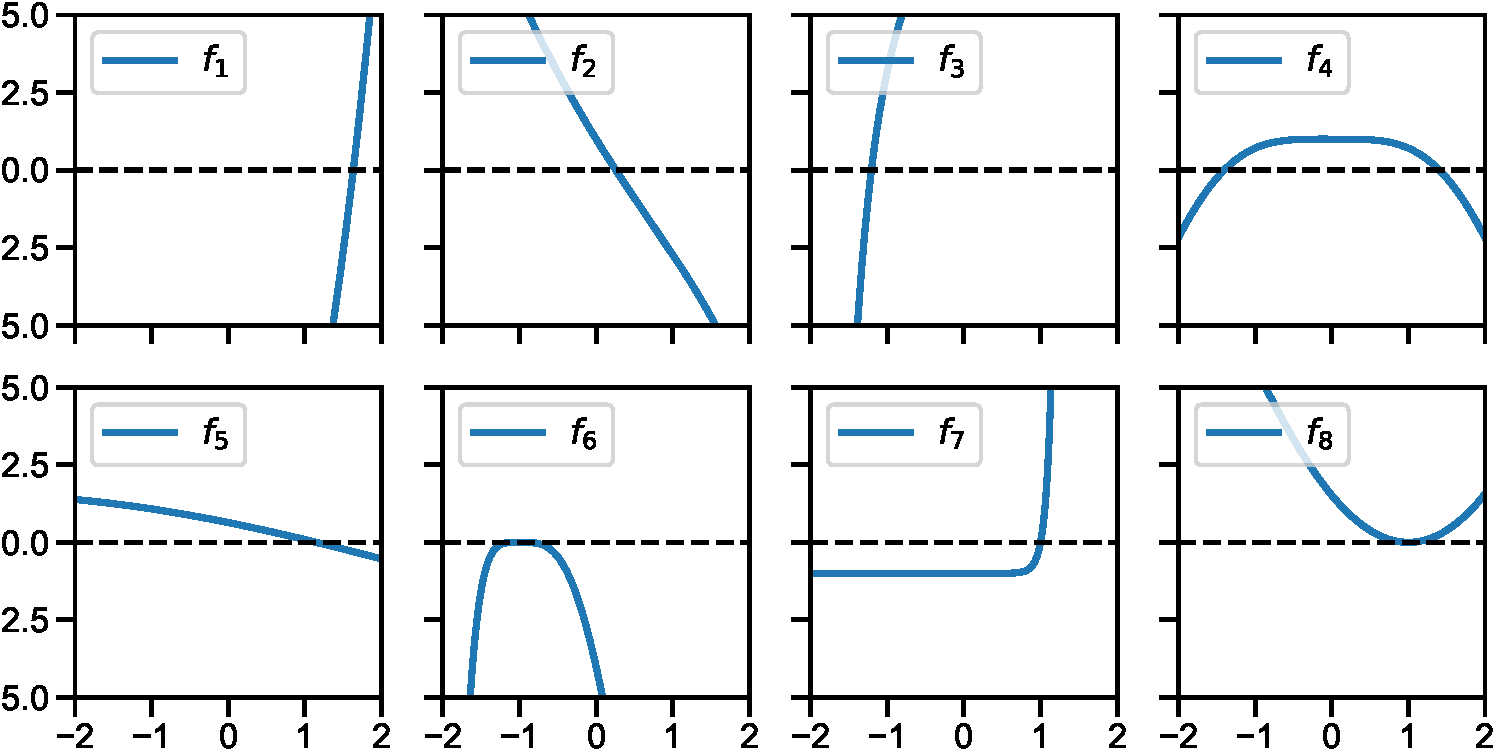
\includegraphics[width=.9\linewidth]{figure/eval-func.pdf}
    \caption{测试函数在零点附近的图像}
    \label{fig:eval-func}
\end{figure}


\subsection{实验结果}

表\ref{tab:exp-result}展示表\ref{tab:compute-eff}的方法对表\ref{tab:eval-func}的函数进行测试的实验结果,对于每个函数都使用了2个分布在根两端的初值进行实验。迭代次数中的$(U)$表示下溢(接近0而超过了精度范围,导致变成0了),$(F)$表示上溢(绝对值太大),$(N)$表示迭代发散。注意IEEE 64位浮点数具有大约15位的规格化有效数字,16位的非规格化有效数字。


\begin{center}
    \begin{longtable}[!htbp]{c|c|ccc|c|c|ccc}
    \caption{迭代次数和误差} \vspace*{-1em} 
    \label{tab:exp-result} \\
    
    \toprule 
    函数 & 初值 & 方法 & \makecell[c]{迭代\\次数} & \makecell[c]{与$x^*$\\误差} & 函数 & 初值 & 方法 & \makecell[c]{迭代\\次数} & \makecell[c]{与$x^*$\\误差} \\ 
    \midrule 
    \endfirsthead
    
    \multicolumn{10}{c}{{\tablename\ \thetable{} 迭代次数和误差(接上页)}} \\
    \toprule 
    函数 & 初值 & 方法 & \makecell[c]{迭代\\次数} & \makecell[c]{与$x^*$\\误差} & 函数 & 初值 & 方法 & \makecell[c]{迭代\\次数} & \makecell[c]{与$x^*$\\误差} \\ 
    \midrule 
    \endhead
    
    \bottomrule 
    \multicolumn{10}{r}{{续下页}} \\
    \endfoot
    
    \bottomrule
    \endlastfoot
    
        \multirow{10}{*}{$f_1$} & 	\multirow{5}{*}{1}  & 	牛顿  & 	6  & 	$-2.22 \cdot 10^{-16}$&	 \multirow{10}{*}{$f_5$}  & 	\multirow{5}{*}{1}  & 	牛顿  & 	4  & 	$2.22 \cdot 10^{-16}$\\

        & 	   & 	Halley  & 	4  & 	$-2.22 \cdot 10^{-16}$&	   & 	   & 	Halley  & 	3  & 	$-2.22 \cdot 10^{-16}$\\
     
        & 	   & 	NM  & 	6  & 	$-4.44 \cdot 10^{-16}$&	   & 	   & 	NM  & 	4  & 	$< 10^{-16}$\\
     
        & 	   & 	GM  & 	3  & 	$-2.22 \cdot 10^{-16}$&	   & 	   & 	GM  & 	3(U)  & 	$\text{-}$\\
     
        & 	   & 	\textbf{本文}  & 	3  & 	$< 10^{-16}$&	   & 	   & 	\textbf{本文}  & 	2  & 	$-2.22 \cdot 10^{-16}$\\
     
     \cline{2-5}\cline{7-10}
        & 	\multirow{5}{*}{2}  & 	牛顿  & 	5  & 	$< 10^{-16}$&	   & 	\multirow{5}{*}{2}  & 	牛顿  & 	5  & 	$-2.22 \cdot 10^{-16}$\\
     
        & 	   & 	Halley  & 	4  & 	$< 10^{-16}$&	   & 	   & 	Halley  & 	4  & 	$< 10^{-16}$\\
     
        & 	   & 	NM  & 	5  & 	$-4.44 \cdot 10^{-16}$&	   & 	   & 	NM  & 	5(U)  & 	$\text{-}$\\
     
        & 	   & 	GM  & 	3  & 	$-2.22 \cdot 10^{-16}$&	   & 	   & 	GM  & 	3(U)  & 	$\text{-}$\\
     
        & 	   & 	\textbf{本文}  & 	3  & 	$-2.22 \cdot 10^{-16}$&	   & 	   & 	\textbf{本文}  & 	3  & 	$-4.44 \cdot 10^{-16}$\\
     
     \cline{2-5}\cline{7-10}
     \hline


    %%%%%%%%%%%%%%%%%%%%%%%%%%%%%%%%%%%%%%%%%%%%%%%%
    % %%%%%%%%%%%% Second row %%%%%%%%%%%%%%%%%%
    %%%%%%%%%%%%%%%%%%%%%%%%%%%%%%%%%%%%%%%%%%%%%%%%
    \multirow{10}{*}{$f_2$} & 	\multirow{5}{*}{0}  & 	牛顿  & 	5  & 	$< 10^{-16}$&	\multirow{10}{*}{$f_6$}   & 	\multirow{5}{*}{-1.5}  & 	牛顿  & 	91  & 	$-2.6 \cdot 10^{-12}$\\

    & 	   & 	Halley  & 	4  & 	$< 10^{-16}$&	   & 	   & 	Halley  & 	53  & 	$-1.01 \cdot 10^{-12}$\\
 
    & 	   & 	NM  & 	4  & 	$< 10^{-16}$&	   & 	   & 	NM  & 	22  & 	$-1.71 \cdot 10^{-13}$\\
 
    & 	   & 	GM  & 	3(U)  & 	$\text{-}$&	   & 	   & 	GM  & 	37  & 	$-8.79 \cdot 10^{-13}$\\
 
    & 	   & 	\textbf{本文}  & 	3  & 	$< 10^{-16}$&	   & 	   & 	\textbf{本文}  & 	38  & 	$-7.74 \cdot 10^{-13}$\\
 
 \cline{2-5}\cline{7-10}
    & 	\multirow{5}{*}{1}  & 	牛顿  & 	5  & 	$< 10^{-16}$&	   & 	\multirow{5}{*}{-0.5}  & 	牛顿  & 	90  & 	$2.32 \cdot 10^{-12}$\\
 
    & 	   & 	Halley  & 	4  & 	$< 10^{-16}$&	   & 	   & 	Halley  & 	52  & 	$1.25 \cdot 10^{-12}$\\
 
    & 	   & 	NM  & 	5  & 	$-2.22 \cdot 10^{-16}$&	   & 	   & 	NM  & 	22  & 	$1.78 \cdot 10^{-13}$\\
 
    & 	   & 	GM  & 	3(U)  & 	$\text{-}$&	   & 	   & 	GM  & 	37  & 	$6.25 \cdot 10^{-13}$\\
 
    & 	   & 	\textbf{本文}  & 	3  & 	$< 10^{-16}$&	   & 	   & 	\textbf{本文}  & 	38  & 	$5.08 \cdot 10^{-13}$\\
 
 \cline{2-5}\cline{7-10}
 \hline



    %%%%%%%%%%%%%%%%%%%%%%%%%%%%%%%%%%%%%%%%%%%%%%%%
    % %%%%%%%%%%%% Third row %%%%%%%%%%%%%%%%%%
    %%%%%%%%%%%%%%%%%%%%%%%%%%%%%%%%%%%%%%%%%%%%%%%%
    \multirow{2}{*}{$f_3$} & 	\multirow{2}{*}{-2}  & 	牛顿  & 	9  & 	$2.22 \cdot 10^{-16}$&	\multirow{2}{*}{$f_7$}    & 	\multirow{2}{*}{0.5}  & 	牛顿  & 	2(F)  & 	$\text{-}$\\

    & 	   & 	Halley  & 	5  & 	$2.22 \cdot 10^{-16}$&	   & 	   & 	Halley  & 	7  & 	$< 10^{-16}$\\

    & 	\multirow{3}{*}{-2}     & 	NM  & 	2(F)  & 	$\text{-}$&	   & 	\multirow{3}{*}{0.5}     & 	NM  & 	2(F)  & 	$\text{-}$\\

    & 	   & 	GM  & 	4  & 	$< 10^{-16}$&	   & 	   & 	GM  & 	2(F)  & 	$\text{-}$\\

    \multirow{4}{*}{$f_3$}& 	   & 	\textbf{本文}  & 	4  & 	$2.22 \cdot 10^{-16}$&	 \multirow{4}{*}{$f_7$}  & 	   & 	\textbf{本文}  & 	2(F)  & 	$\text{-}$\\

\cline{2-5}\cline{7-10}
    & 	\multirow{5}{*}{-1}  & 	牛顿  & 	6  & 	$2.22 \cdot 10^{-16}$&	   & 	\multirow{5}{*}{1.5}  & 	牛顿  & 	12  & 	$-1.11 \cdot 10^{-16}$\\

    & 	   & 	Halley  & 	4  & 	$2.22 \cdot 10^{-16}$&	   & 	   & 	Halley  & 	7  & 	$-1.11 \cdot 10^{-16}$\\

    & 	   & 	NM  & 	7  & 	$-1.02 \cdot 10^{-14}$&	   & 	   & 	NM  & 	2(F)  & 	$\text{-}$\\

    & 	   & 	GM  & 	3  & 	$< 10^{-16}$&	   & 	   & 	GM  & 	5  & 	$< 10^{-16}$\\

    & 	   & 	\textbf{本文}  & 	3  & 	$2.22 \cdot 10^{-16}$&	   & 	   & 	\textbf{本文}  & 	6  & 	$< 10^{-16}$\\

\cline{2-5}\cline{7-10}
\hline




    %%%%%%%%%%%%%%%%%%%%%%%%%%%%%%%%%%%%%%%%%%%%%%%%
    % %%%%%%%%%%%% Forth row %%%%%%%%%%%%%%%%%%
    %%%%%%%%%%%%%%%%%%%%%%%%%%%%%%%%%%%%%%%%%%%%%%%%
    \multirow{10}{*}{$f_4$} & 	\multirow{5}{*}{1}  & 	牛顿  & 	6  & 	$< 10^{-16}$&	\multirow{10}{*}{$f_8$}    & 	\multirow{5}{*}{0.5}  & 	牛顿  & 	39  & 	$-9.01 \cdot 10^{-13}$\\

    & 	   & 	Halley  & 	4  & 	$2.22 \cdot 10^{-16}$&	   & 	   & 	Halley  & 	26  & 	$-1.96 \cdot 10^{-13}$\\

    & 	   & 	NM  & 	7  & 	$2.22 \cdot 10^{-16}$&	   & 	   & 	NM  & 	27(N)  & 	$-4.0$\\

    & 	   & 	GM  & 	3  & 	$< 10^{-16}$&	   & 	   & 	GM  & 	17  & 	$-2.18 \cdot 10^{-13}$\\

    & 	   & 	\textbf{本文}  & 	3  & 	$< 10^{-16}$&	   & 	   & 	\textbf{本文}  & 	16  & 	$-1.75 \cdot 10^{-13}$\\

\cline{2-5}\cline{7-10}
    & 	\multirow{5}{*}{2}  & 	牛顿  & 	6  & 	$< 10^{-16}$&	   & 	\multirow{5}{*}{1.5}  & 	牛顿  & 	39  & 	$9.14 \cdot 10^{-13}$\\

    & 	   & 	Halley  & 	4  & 	$2.22 \cdot 10^{-16}$&	   & 	   & 	Halley  & 	26  & 	$1.97 \cdot 10^{-13}$\\

    & 	   & 	NM  & 	7  & 	$2.22 \cdot 10^{-16}$&	   & 	   & 	NM  & 	14(N)  & 	$-4.0$\\

    & 	   & 	GM  & 	3  & 	$< 10^{-16}$&	   & 	   & 	GM  & 	17  & 	$2.19 \cdot 10^{-13}$\\

    & 	   & 	\textbf{本文}  & 	3  & 	$< 10^{-16}$&	   & 	   & 	\textbf{本文}  & 	16  & 	$1.78 \cdot 10^{-13}$\\

    \end{longtable}
\end{center}


\subsection{结果分析}


表\ref{tab:exp-summary}总结了这5种方法的成功次数和失败原因。Halley法在所有测试中均成功得到结果,这可能是因为它使用了二阶导数,数值稳定性非常好。牛顿法和本方法除了有一次上溢以外也都成功了。GM法出现了4次下溢错误,这是因为它的公式中包含“小数减小数”、“小数除小数”等计算,因此非常容易产生下溢,数值稳定性不好。NM法中出现了3次上溢和2次发散,这可能是因为它每代额外使用7次乘除法,加速了误差积累。本方法作为六阶收敛的方法,数值稳定性与牛顿法相当,高于另外两种方法,且计算效率(公式\ref{eq:EI})高于牛顿法,具有良好的实用价值。

对前5个函数$f_1\sim f_5$,各方法基本有比较好的效果,并且迭代次数趋势也与收敛阶相匹配。对于第6个函数$f_6$,其\textbf{零点是4重根},因此牛顿法收敛速度非常慢,NM法最快,GM法和本方法相当。对于第7个函数$f_7$,选取初值$x_0=0.5$时,多种方法均产生了上溢,观察函数图像(图\ref{fig:eval-func})发现它在$(-2, 1]$上非常平缓,因此\textbf{导数很小,基于牛顿法的一系列方法在计算$\dfrac{f(x_n)}{f'(x_n)}$时容易上溢}。但是当选取另一个初值$x_0=1.5$时,由于导数很大,因此没有这个问题。对于第8个函数$f_8$,NM很意外的发散了,因此及时终止了迭代,由于时间有限我没有仔细探究其原因。由于\textbf{零点是2重根}的原因,牛顿法同样收敛的很慢,但本方法拥有最快的收敛速度,GM法其次。



\begin{table}[!htbp]
    \centering
    \caption{各方法成功次数和失败原因}
    \label{tab:exp-summary}
    \begin{tabular}{c|ccccc}
        \toprule
        类型 & 牛顿 & \makecell[c]{Halley\\(公式\ref{eq:real-halley})} & \makecell[c]{NM\cite{neta1979sixth}\\(公式\ref{eq:NM})} & \makecell[c]{GM\cite{grau2006improvement}\\(公式\ref{eq:GM})} & \makecell[c]{本文\\(公式\ref{eq:my})} \\
        \midrule
        成功 & 15 & 16 & 10 & 12 & 15 \\
        下溢 & 0  & 0  & 1  & 3  & 0 \\
        上溢 & 1  & 0  & 3  & 1  & 1 \\
        发散 & 0  & 0  & 2  & 0  & 0 \\
        \bottomrule
    \end{tabular}
\end{table}



\subsection{对重根的讨论}

计算收敛阶(COC, Computational order of convergence)\cite{cordero2007variants}是数值方法在实际计算过程中的收敛阶,其定义如下:
\begin{equation}
    COC = \dfrac{\ln\left( \left| \dfrac{x_{n+1} - x_n}{x_n - x_{n-1}} \right| \right)}{\ln\left( \left| \dfrac{x_n - x_{n-1}}{x_{n-1} - x_{n-2}} \right| \right)}
\end{equation}
表\ref{tab:coc}所示本文列举了$f_6 \sim f_8$的计算收敛阶。对于单根的函数$f_7$,各方法的计算收敛阶基本符合其理论的收敛阶;对于重根函数$f_6$和$f_8$,所有方法只有线性收敛。

\begin{table}[!htbp]
    \centering
    \caption{计算重根时的COC}
    \label{tab:coc}
    \begin{tabular}{cc|c|ccccc}
        \toprule
        函数 & 重复度 & 初值 & 牛顿 & Halley & NM & GM & 本文 \\
        \midrule
        $f_7$ & 单根 & 1.5 & 2.002 & 3.066 & 发散  & 5.990 & 6.053 \\
        \hline
        \multirow{2}{*}{$f_6$} & \multirow{2}{*}{4重根}
        & -1.5 & 0.991 & 0.998 & 1.000  & 0.985 & 0.993 \\
        & & -0.5 & 0.996 & 0.996 & 0.999  & 1.001 & 1.000 \\
        \hline
        \multirow{2}{*}{$f_8$} & \multirow{2}{*}{2重根}
        & 0.5 & 1.000 & 0.998 & 发散  & 1.000 & 1.000 \\
        &  & 1.5 & 0.977 & 1.021 & 发散  & 1.000 & 0.999 \\
        \bottomrule
    \end{tabular}
\end{table}

为了加速对重根的收敛,使用PPT第43页对迭代公式进行改造:
\begin{equation}
    \label{eq:my-m}
    \begin{cases}
        y_n &= x_n - m \cdot \dfrac{f(x)}{f'(x)} \\
        z_n &= x_n - \dfrac{2f(x_n)}{f'(x_n) + f'(y_n)} \\
        x_{n+1} &= z_n - m \cdot \dfrac{f(z_n)}{f'(z_n)},
    \end{cases}
\end{equation}
其中$m$是重根次数,同时采用类似方法对GM进行改造。由于时间关系因此没有对改造后的收敛阶进行证明。使用新的迭代公式对具有4阶重根的$f_6$进行实验并考察COC,表\ref{tab:multi-root}展示了实验迭代过程。可以发现这种朴素的改造方法其实只是和牛顿法等效,并没有实现它应有的六阶收敛。因此能保持六阶收敛的对重根的迭代法仍然需要经过推导才能得到,不能这样简单的模仿。


\begin{table}[!htbp]
    \centering
    \caption{加速重根收敛实验结果}
    \label{tab:multi-root}
    \begin{tabular}{c|ccc}
        \toprule
        n & 牛顿 & GM & 本文 \\
        \midrule
        1 &  -1.0643564356435644 &  -1.0642142761848583 &  -1.0218785203047935 \\
        2 &  -1.0012164573169233 &  -1.0012111303753073 &  -1.0000362366521056 \\
        3 &  -1.0000004437505903 &  -1.0000004398734581 &  -1.0000000000984837 \\
        4 &  -1.0000000000000591 &  -1.0000000000000580 &  -1.0000000000000000 \\
        5 &  -1.0000000000000000 &  -1.0000000000000000 &                  - \\
        \bottomrule
        COC & 2.000 & 2.000 & 2.002 \\
        \bottomrule
    \end{tabular}
\end{table}






\subsection{部分函数迭代过程展示(作为补充材料)}

% 作为补充材料,表\ref{tab:f4}和表\ref{tab:f7}对一些函数的迭代过程进行了展示。

\begin{table}[!htbp]
    \centering
    \caption{$f_4$选取初值为2的迭代过程}
    \label{tab:f4}
    \hspace*{-3em}
    \begin{tabular}{c|ccccc}
        \toprule
        $n$ &             牛顿 &             Halley &               NM &               GM &               本文 \\
        \midrule
        0 & 2 & 2 & 2 & 2 & 2 \\
        1 &  1.543143068960336 &  1.456885216221384 &  1.120415325387814 &  1.407237330215151 &  1.405535212978439 \\
        2 &  1.417094222312942 &  1.404562548049610 &  1.309731172778497 &  1.404491648215341 &  1.404491648215341 \\
        3 &  1.404614018363034 &  1.404491648215529 &  1.397104012247177 &  1.404491648215341 &  1.404491648215341 \\
        4 &  1.404491659946959 &  1.404491648215341 &  1.404448806412075 &                - &                - \\
        5 &  1.404491648215341 &                - &  1.404491646777146 &                - &                - \\
        6 &  1.404491648215341 &                - &  1.404491648215341 &                - &                - \\
        \bottomrule
    \end{tabular}
\end{table}




\begin{table}[!htbp]
    \centering
    \caption{$f_7$选取初值为1.5的迭代过程}
    \label{tab:f7}
    \hspace*{-3em}
    \begin{tabular}{c|ccccc}
        \toprule
        & 牛顿 & Halley & NM & GM & \textbf{本文} \\
        \midrule
        0 & 1.5 & 1.5 & 1.5 & 1.5 & 1.5 \\
        1  &  1.428655062830056 &  1.356011165775886 &                                  0.666554094953474 &  1.302765996348761 &  1.323425736359648 \\
        2  &  1.356719234358469 &  1.211129011680508 &  $-1.275596982 \cdot 10^{52}$ &  1.109913322973212 &  1.147701833153800 \\
        3  &  1.284419811223503 &  1.078073976922075 &                                                - &  1.002996956434495 &  1.017028589466088 \\
        4  &  1.212406308451123 &  1.006179477275287 &                                                - &  1.000000000003765 &  1.000000403894250 \\
        5  &  1.142418159478025 &  1.000003327216270 &                                                - &  1.000000000000000 &  1.000000000000000 \\
        6  &  1.078725914448773 &  1.000000000000000 &                                                - &                - &  1.000000000000000 \\
        7  &  1.029866713280862 &  1.000000000000000 &                                                - &                - &                - \\
        8  &  1.005182160439837 &                - &                                                - &                - &                - \\
        9  &  1.000172764038992 &                - &                                                - &                - &                - \\
        10 &  1.000000196158916 &                - &                                                - &                - &                - \\
        11 &  1.000000000000253 &                - &                                                - &                - &                - \\
        12 &  1.000000000000000 &                - &                                                - &                - &                - \\
        \bottomrule
    \end{tabular}
\end{table}